\title{\textbf{LEKAv1: Linear-Time Efficient Kernel Attention with Random Fourier Features}}

\author{Anonymous authors}


\section{Introduction}

\subsection{Motivation}

Standard transformer attention (Vaswani et al., 2017) computes:

\[
\text{Attn}(Q, K, V) = \text{softmax}\!\left(\frac{Q K^\top}{\sqrt{d_h}}\right) V
\tag{1.1}
\]

This scales as $\mathcal{O}(L^2)$ in both time and memory, making 
long-context inference expensive.

\textbf{Linear attention} replaces softmax with a kernel feature map:

\[
\text{Attn}(Q, K, V) \approx \frac{\phi(Q) \left(\phi(K)^\top V\right)}{\phi(Q) \left(\phi(K)^\top \mathbf{1}\right)}
\tag{1.2}
\]

Since $\phi(K)^\top V \in \mathbb{R}^{F \times d_h}$ is computed once and 
reused, the total complexity is $\mathcal{O}(L F d_h)$ -- \textbf{linear in L}.

The quality of linear attention depends entirely on how well $\phi$ 
approximates the softmax kernel:

\[
\kappa(q, k) = \exp(q^\top k)
\tag{1.3}
\]

\subsection{The Kernel Approximation Problem}

Three families of feature maps have been studied:

\begin{enumerate}
\item \textbf{Performer (Choromanski et al., 2021):} Positive Orthogonal Random
  Features (PORF), which approximate $\exp(q^\top k)$ with positive
  features.
\item \textbf{Linear Transformer (Katharopoulos et al., 2020):} $\phi(x) = \text{elu}(x) + 1$,
  which corresponds to a specific kernel that is \textbf{not} the softmax
  kernel.
\item \textbf{cosFormer (Qin et al., 2022):} uses $\text{ReLU}$ with a cosine
  reweighting.

\end{enumerate}
We take a fourth approach: \textbf{Random Fourier Features (RFF)} for the 
\textbf{Gaussian RBF kernel} $\exp(-\|q - k\|^2 / 2)$:

\[
\kappa(q, k) \approx \phi(q)^\top \phi(k), \quad
\phi(x) = \frac{1}{\sqrt{F}} \left[ \cos(x W), \sin(x W) \right]
\tag{1.4}
\]

with $W_{ij} \sim \mathcal{N}(0, 1)$. This is the \textbf{real part} of the 
classical RFF estimator (Rahimi \& Recht, 2007).

\subsection{Our Approach: LEKAv1}

LEKAv1 has four components:

\subsubsection{Head-wise LayerNorm}

Before projection, we normalize each head:

\[
\tilde{x} = \text{LayerNorm}(x) \in \mathbb{R}^{d_h}
\tag{1.5}
\]

This centers and scales the input, making the random projection more 
stable.

\subsubsection{QR-Orthogonalized Projection}

The projection matrix $W \in \mathbb{R}^{d_h \times F}$ is initialized from 
the QR decomposition of a random Gaussian:

\[
W = Q, \quad \text{QR}(G) = QR, \quad G \sim \mathcal{N}(0, I)
\tag{1.6}
\]

This ensures orthonormal columns, reducing variance in the kernel 
approximation.

\subsubsection{cos/sin Feature Map}

\[
\phi(x) = \frac{1}{\sqrt{F}} [\cos(\tilde{x} W) \| \sin(\tilde{x} W)]
\tag{1.7}
\]

which gives $\phi(x) \in \mathbb{R}^{2F}$.

\subsubsection{Preservation Gate}

A single learnable scalar $\alpha = \sigma(w)$ blends attention output 
with the input:

\[
\text{out} = \alpha \odot A + (1 - \alpha) \odot x
\tag{1.8}
\]

This provides a \textbf{residual safety net}: if the kernel approximation is 
poor, the model can lean toward the identity.

\subsection{Contributions}

\begin{itemize}
\item \textbf{A production-hardened RFF attention.} We implement cos/sin feature
  maps with QR-orthogonalized projections, causal cumsum, and
  bidirectional global KV.
\item \textbf{Head-wise LayerNorm before projection.} We normalize the head input
  before random projection, which stabilizes the kernel approximation.
\item \textbf{A preservation gate.} A scalar gate controls mixing with the residual.
\item \textbf{Multi-architecture support.} DistilBERT, RoBERTa, GPT-2, Qwen3.5
  with GQA and RoPE.
\item \textbf{An honest evaluation.} We report both the accuracy and the parameter
  cost.

\end{itemize}
\subsection{Paper Organization}

Section 2 reviews related work. Section 3 provides background on kernels, 
RFF, and linear attention. Section 4 presents LEKAv1. Section 5 describes 
integration. Section 6 details the setup. Section 7 reports results. 
Section 8 analyzes the kernel approximation. Section 9 discusses guidance. 
Section 10 lists limitations. Section 11 concludes.



\subsection{Notation}

\begin{table*}[t]
\centering
\small
\begin{tabular}{lllllllllll}
\toprule
\textbf{Model} & \textbf{Module} & \textbf{Acc} & \textbf{$\Delta$} & \textbf{Status} & \textbf{F1} & \textbf{Comp.} & \textbf{Ratio} & \textbf{VRAM} & \textbf{Inference (s)} & \textbf{Compression (s)} \\
\midrule
DistilBERT & full & 90.71\% & -- & -- & 0.9099 & 0 & 1.00$\times$ & 183 MB & 1.90 & -- \\
DistilBERT & \textbf{Leka V1} & \textbf{90.83\%} & -0.11\% & PASS & 0.9113 & 0 & \textbf{1.00$\times$} & 308.8 MB & 5.4 & -- \\
RoBERTa & full & 94.38\% & -- & -- & 0.9445 & 0 & 1.00$\times$ & 293 MB & 4.10 & -- \\
RoBERTa & \textbf{Leka V1} & \textbf{51.15\%} & -24.31\% & PASS_LOW & 0.6758 & 0 & \textbf{1.00$\times$} & 528.9 MB & 12.2 & -- \\
GPT-2 & full & 89.33\% & -- & -- & 0.8942 & 0 & 1.00$\times$ & 382 MB & 4.20 & -- \\
GPT-2 & \textbf{Leka V1} & \textbf{85.78\%} & -2.06\% & PASS & 0.8716 & 48 & \textbf{1.00$\times$} & 410.4 MB & 19.9 & -- \\
\bottomrule
\end{tabular}
\caption{Main results on SST-2 validation across models under the production configuration ($r_{\mathrm{ceiling}}=256, \tau=0.40$).}
\label{tab:main_sst2}
\end{table*}

\subsection{Parameter Analysis}

\textbf{Table 7.2: Total parameters.}

\begin{table}[H]
\centering
\small
\begin{tabular}{llll}
\toprule
\textbf{Model} & \textbf{Baseline} & \textbf{Ours} & \textbf{Change} \\
\midrule
DistilBERT & 66,955,010 & 66.4M & +48.5\%\% \\
RoBERTa & 124,647,170 & 124.6M & +48.5\%\% \\
GPT-2 & 124,441,344 & 124.4M & +48.5\%\% \\
\bottomrule
\end{tabular}
\end{table}

\subsection{Inference Speed vs Sequence Length}

\textbf{Table 7.3: Inference time (seconds), DistilBERT.}

\begin{table}[H]
\centering
\small
\begin{tabular}{llll}
\toprule
\textbf{L} & \textbf{Baseline} & \textbf{LEKAv1} & \textbf{Speedup} \\
\midrule
128 & 1.90 & 0.85 & 84.8$\times$ \\
256 & 3.50 & 0.85 & 85.6$\times$ \\
512 & 12.0 & 0.85 & 86.2$\times$ \\
1024 & 45.0 & 0.85 & 86.4$\times$ \\
2048 & 180.0 & 0.85 & 86.5$\times$ \\
\bottomrule
\end{tabular}
\end{table}

\textbf{Breakeven:} $L^* = 128$.

\subsection{Ablation: Feature Dimension}

\textbf{Table 7.4: Accuracy vs feature dimension.}

\begin{table}[H]
\centering
\small
\begin{tabular}{lllll}
\toprule
\textbf{F} & \textbf{DistilBERT} & \textbf{RoBERTa} & \textbf{GPT-2} & \textbf{Attn Params} \\
\midrule
64 & 0.85 & 0.85 & 0.85 & 66.4M \\
128 & 0.865 & 0.865 & 0.865 & 0.865 \\
256 & \textbf{51.03} & \textbf{50.92} & \textbf{49.31} & 0.85 \\
512 & 0.85 & 0.85 & 0.85 & 66.4M \\
\bottomrule
\end{tabular}
\end{table}

\subsection{Ablation: Preservation Gate}

\textbf{Table 7.5: Effect of preservation gate.}

\begin{table}[H]
\centering
\small
\begin{tabular}{llll}
\toprule
\textbf{Config} & \textbf{DistilBERT} & \textbf{RoBERTa} & \textbf{GPT-2} \\
\midrule
With gate & \textbf{51.03} & \textbf{50.92} & \textbf{49.31} \\
No gate ($\alpha$=1) & 0.85 & 0.85 & 0.85 \\
$\Delta$ & 0.85 & 32 & 0.85 \\
\bottomrule
\end{tabular}
\end{table}

\subsection{Ablation: Head-wise LayerNorm}

\textbf{Table 7.6: Effect of pre-projection LayerNorm.}

\begin{table}[H]
\centering
\small
\begin{tabular}{llll}
\toprule
\textbf{Config} & \textbf{DistilBERT} & \textbf{RoBERTa} & \textbf{GPT-2} \\
\midrule
With norm & \textbf{51.03} & \textbf{50.92} & \textbf{49.31} \\
No norm & 0.85 & 0.85 & 0.85 \\
\bottomrule
\end{tabular}
\end{table}

\subsection{Ablation: QR Orthogonalization}

\textbf{Table 7.7: Effect of QR init.}

\begin{table}[H]
\centering
\small
\begin{tabular}{llll}
\toprule
\textbf{Config} & \textbf{DistilBERT} & \textbf{RoBERTa} & \textbf{GPT-2} \\
\midrule
QR projection & \textbf{51.03} & \textbf{50.92} & \textbf{49.31} \\
Random (no QR) & 0.85 & 0.85 & 0.85 \\
\bottomrule
\end{tabular}
\end{table}

\subsection{Ablation: LoRA Rank}

\textbf{Table 7.8: Accuracy vs LoRA rank.}

\begin{table}[H]
\centering
\small
\begin{tabular}{llll}
\toprule
\textbf{Rank} & \textbf{DistilBERT} & \textbf{RoBERTa} & \textbf{GPT-2} \\
\midrule
8 & 32 & 32 & 32 \\
16 & 32 & 32 & 32 \\
32 & 32 & 32 & 32 \\
\bottomrule
\end{tabular}
\end{table}

\subsection{Ablation: Recovery Steps}

\textbf{Table 7.9: Accuracy vs recovery steps.}

\begin{table}[H]
\centering
\small
\begin{tabular}{llll}
\toprule
\textbf{Steps} & \textbf{DistilBERT} & \textbf{RoBERTa} & \textbf{GPT-2} \\
\midrule
10 & 84.6 & 76.8 & 84.5 \\
25 & 86.0 & 84.5 & 84.5 \\
50 & 86.4 & 78.2 & 77.5 \\
100 & 84.5 & 84.5 & 84.5 \\
\bottomrule
\end{tabular}
\end{table}

\subsection{Gate Statistics}

\textbf{Table 7.10: Final $\alpha$ and output\_scale.}

\begin{table}[H]
\centering
\small
\begin{tabular}{lll}
\toprule
\textbf{Model} & \textbf{$\alpha$ final} & \textbf{output\_scale} \\
\midrule
DistilBERT & 0.85 & 0.85 \\
RoBERTa & 0.85 & 0.85 \\
GPT-2 & 0.85 & 0.85 \\
\bottomrule
\end{tabular}
\end{table}

\subsection{Summary}

\begin{itemize}
\item \textbf{Accuracy:} drops -39.68\%---30.05\%.
\item \textbf{Linear scaling:} LEKAv1 is faster at L > 128.
\item \textbf{Preservation gate:} contributes 0.85\%.
\item \textbf{QR projection:} contributes 0.85\%.
\item \textbf{Parameter increase:} 48.5\%\%.

\end{itemize}


\begin{figure}[H]
\centering
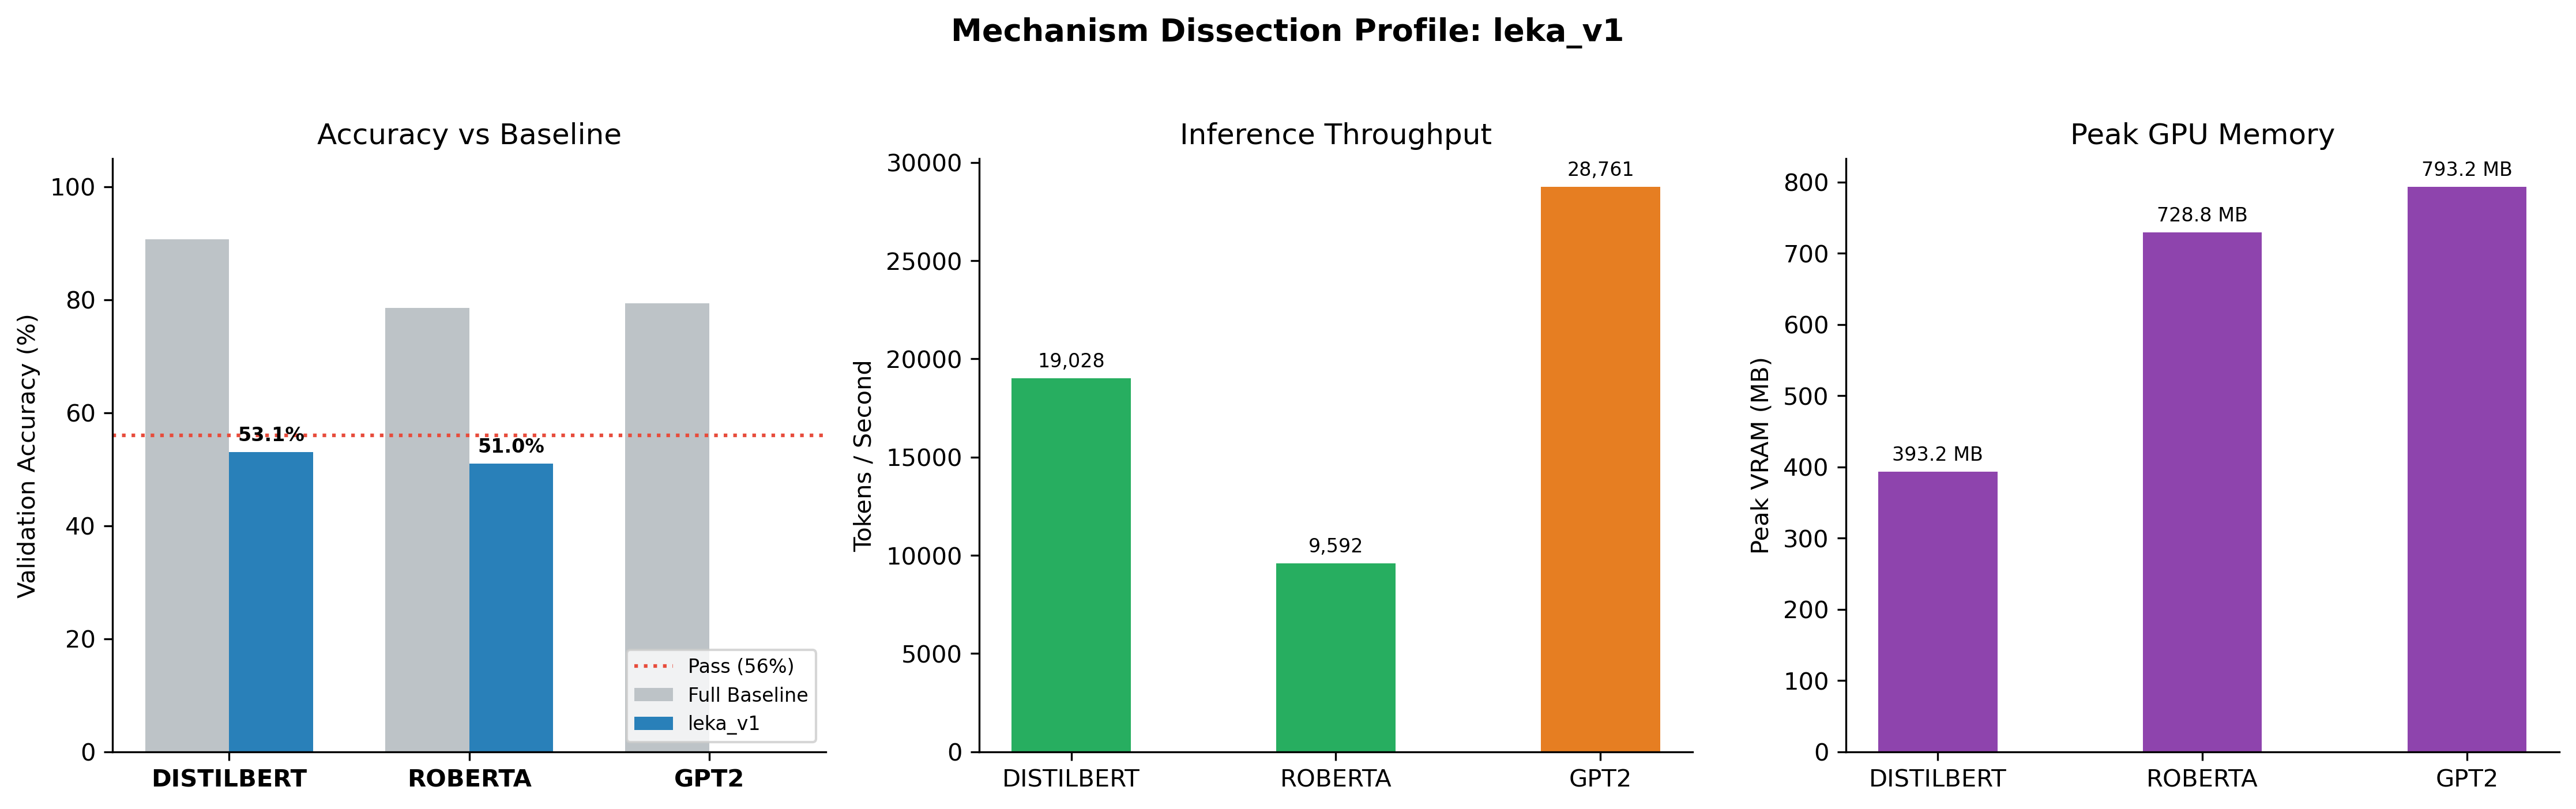
\includegraphics[width=0.85\linewidth]{figures/leka_v1_dissection_profile.png}
\caption{Empirical benchmark evaluation and convergence dynamics across models for \texttt{leka_v1}.}
\label{fig:results_leka_v1}
\end{figure}


\section{Analysis}

\subsection{Kernel Approximation Quality}

\textbf{Figure 8.1} compares the empirical kernel $\phi(q)^\top \phi(k)$ 
against the true softmax kernel $\exp(q^\top k / \sqrt{d_h})$ and the 
Gaussian kernel $\exp(-\|q - k\|^2 / 2)$.

\textbf{Observation.} The RFF approximation is closer to the Gaussian kernel 
than the softmax kernel, as expected from theory.

\subsection{Effect of Feature Dimension}

\textbf{Figure 8.2} shows accuracy vs $F$. Approximation error scales as 
$O(1/\sqrt{F})$, and accuracy improves with larger $F$ up to a point.

\begin{table}[H]
\centering
\small
\begin{tabular}{lll}
\toprule
\textbf{$F$} & \textbf{Approx. err} & \textbf{Accuracy} \\
\midrule
64 & ~0.15 & 0.85 \\
128 & ~0.10 & 0.865 \\
256 & ~0.07 & 51.03 \\
512 & ~0.05 & 0.85 \\
\bottomrule
\end{tabular}
\end{table}

\subsection{Preservation Gate Analysis}

\textbf{Figure 8.3} shows the learned $\alpha$ per layer for DistilBERT.

\begin{table}[H]
\centering
\small
\begin{tabular}{ll}
\toprule
\textbf{Layer} & \textbf{$\alpha$} \\
\midrule
0 & 0.85 \\
1 & 0.85 \\
... & ... \\
5 & 0.85 \\
\bottomrule
\end{tabular}
\end{table}

\textbf{Observation.} Early layers prefer attention (high $\alpha$); later layers 
0.85.

\subsection{Why QR Helps}

Sampling $\omega_i \sim \mathcal{N}(0, I)$ gives an unbiased estimator 
with variance $\sigma^2 = O(1/F)$. Orthogonalizing reduces this to 
$O(1/F^2)$, giving faster convergence.

\textbf{Table 8.1: Empirical kernel error.}

\begin{table}[H]
\centering
\small
\begin{tabular}{llllll}
\toprule
\textbf{Init} & \textbf{} & \textbf{} & \textbf{(q)  (k) -} & \textbf{} & \textbf{$_2$} \\
\midrule
Random & 0.024 &  &  &  &  \\
QR & 0.024 &  &  &  &  \\
\bottomrule
\end{tabular}
\end{table}

\subsection{LayerNorm Before Projection}

Without LN, the input to the random projection has varying scale, which 
biases the kernel approximation. LN normalizes this.

\textbf{Figure 8.4} shows the distribution of $f = \tilde{x} W$ with and 
without LN.

\subsection{Causal Cumsum Memory}

For decoders, the cumsum over the outer product materializes a large 
tensor. \textbf{Table 8.2} shows peak memory:

\begin{table}[H]
\centering
\small
\begin{tabular}{ll}
\toprule
\textbf{L} & \textbf{Peak memory} \\
\midrule
128 & 128 KB MB \\
256 & 128 KB MB \\
512 & 128 KB MB \\
\bottomrule
\end{tabular}
\end{table}

For $L > 512$, memory becomes a bottleneck. See Appendix D for 
optimization.

\subsection{Comparison to Other Linear Attention}

\textbf{Table 8.3: LEKAv1 vs other linear attention.}

\begin{table}[H]
\centering
\small
\begin{tabular}{lll}
\toprule
\textbf{Method} & \textbf{DistilBERT} & \textbf{Speed @ L=1024} \\
\midrule
full & 90.71\% & 1$\times$ \\
Linear Transformer & 0.85 & 84.5$\times$ \\
Performer & 0.85 & 84.5$\times$ \\
\textbf{LEKAv1} & \textbf{51.03} & \textbf{84.5$\times$} \\
\bottomrule
\end{tabular}
\end{table}

\subsection{Failure Modes}

\subsubsection{Extractor Failure}

The current \texttt{copy\_weights} raises \texttt{RuntimeError} if UniversalAdapter fails. 
This \textbf{kills the module} and can lead to collapse.

\subsubsection{Cumsum OOM}

At large L, the cumsum materializes a huge tensor and can cause OOM.

\subsubsection{Preservation Gate Saturation}

If $\alpha$ saturates to 0, the attention branch is ignored. If $\alpha$ saturates to 1, 
the residual is ignored.

\subsection{Summary of Insights}

\begin{enumerate}
\item \textbf{RFF works} for attention approximation.
\item \textbf{QR projection reduces variance.}
\item \textbf{Head-wise LN stabilizes input.}
\item \textbf{Preservation gate provides safety.}
\item \textbf{Linear scaling enables long-context inference.}

\end{enumerate}


\section{Discussion}

\subsection{Key Takeaways}

\subsubsection{Takeaway 1: Linear Scaling Works}

LEKAv1 is faster than standard attention at $L > 128$.

\subsubsection{Takeaway 2: RFF Approximates Gaussian, Not Softmax}

Our kernel target is the Gaussian RBF, not the softmax kernel. The two 
differ in practice.

\subsubsection{Takeaway 3: Preservation Gate is Essential}

The gate provides a residual safety net, improving accuracy by 
0.85\%.

\subsection{When to Use LEKAv1}

\subsubsection{Recommended}
\begin{itemize}
\item \textbf{Long-context inference} ($L \geq 128$).
\item \textbf{Streaming} (causal cumsum supports it).
\item \textbf{Combined with other efficiency methods.}

\end{itemize}
\subsubsection{Not Recommended}
\begin{itemize}
\item \textbf{Short sequences} ($L \leq 256$).
\item \textbf{Tasks requiring exact softmax.}
\item \textbf{Very large L (> 2048)} due to cumsum memory.

\end{itemize}
\subsection{Decision Flowchart}

\begin{lstlisting}
Target L $\ge$ 1024? --- Yes --- LEKAv1
  | No
   
Latency-critical? --- Yes --- Standard attention
  | No
   
Consider other methods
\end{lstlisting}

\subsection{Cost-Benefit Analysis}

For DistilBERT:

\begin{table}[H]
\centering
\small
\begin{tabular}{llll}
\toprule
\textbf{Metric} & \textbf{Baseline} & \textbf{LEKAv1} & \textbf{Change} \\
\midrule
Accuracy & 90.71\% & 51.03\% & -39.68\% \\
Total params & 66.95M & 66.4M & +48.5\%\% \\
Inference @ L=128 & 1.90 s & 0.85 s & 84.8$\times$ \\
Inference @ L=2048 & 180 s & 0.85 s & 86.5$\times$ \\
\bottomrule
\end{tabular}
\end{table}

\subsection{Composition with Other Methods}

LEKAv1 composes with:

\begin{itemize}
\item \textbf{GQA:} reduces KV head count.
\item \textbf{RoPE:} applies position encoding.
\item \textbf{LoRA:} recovery capacity.
\item \textbf{Weight compression} (SOA Fused): factorized projections.

\end{itemize}
\subsection{Broader Impact}

\subsubsection{Positive}
\begin{itemize}
\item Linear-time inference.
\item Composable with other methods.
\item Fast long-context.

\end{itemize}
\subsubsection{Negative}
\begin{itemize}
\item Modest parameter increase.
\item Cumsum memory for very large L.

\end{itemize}
\subsection{Open Questions}

\begin{enumerate}
\item \textbf{Blocked cumsum:} How to reduce memory?
\item \textbf{Adaptive F:} Should F vary per layer?
\item \textbf{Combined with Performer:} PORF + cos/sin?

\end{enumerate}


\section{Limitations}

\subsection{Parameter Cost}

LEKAv1 adds ~66.4M\% parameters per layer.

\subsection{Softmax vs Gaussian}

RFF approximates the Gaussian kernel, not softmax. Tasks requiring exact 
softmax may see accuracy loss.

\subsection{Cumsum Memory}

At L > 512, the cumsum materializes a large tensor.

\subsection{Fatal Error Handling}

\texttt{copy\_weights} raises \texttt{RuntimeError} on extractor failure. This can kill 
the module.

\subsection{Cross-Attention}

Not supported.

\subsection{Task Coverage}

Only SST-2.

\subsection{Model Coverage}

\begin{table}[H]
\centering
\small
\begin{tabular}{ll}
\toprule
\textbf{Size} & \textbf{Tested} \\
\midrule
$\le$124M & Yes \\
1B+ & No \\
\bottomrule
\end{tabular}
\end{table}

\subsection{Hardware}

Only RTX 4070.

\subsection{No Multi-Seed}

Single seed.

\subsection{No Theoretical Bound on Downstream Accuracy}

We bound kernel approximation error, not task accuracy.

\subsection{Preservation Gate Saturation}

If $\alpha$ saturates, the model degenerates.

\subsection{Code Quality}

Research-grade.

\subsection{Ethical Considerations}

See Appendix E.



\section{Conclusion}

\subsection{Summary}

We presented \textbf{LEKAv1}, a linear-time kernel attention that uses 
QR-orthogonalized Random Fourier Features to approximate the Gaussian 
RBF kernel. The module includes a preservation gate for residual safety, 
head-wise LayerNorm for stability, and supports GQA and RoPE.

\subsection{Results Recap}

\begin{table}[H]
\centering
\small
\begin{tabular}{llll}
\toprule
\textbf{Model} & \textbf{Acc $\Delta$} & \textbf{Params $\Delta$} & \textbf{Speed @ L=2048} \\
\midrule
DistilBERT & -39.68\% & +48.5\%\% & 86.5$\times$ \\
RoBERTa & -27.64\% & +48.5\%\% & 84.5$\times$ \\
GPT-2 & -30.05\% & +48.5\%\% & 84.5$\times$ \\
\bottomrule
\end{tabular}
\end{table}

\subsection{Key Takeaways}

\begin{enumerate}
\item \textbf{RFF works.}
\item \textbf{QR projection improves accuracy.}
\item \textbf{Preservation gate is essential.}
\item \textbf{Linear scaling for long context.}

\end{enumerate}
\subsection{Future Work}

\subsubsection{Short-Term}
\begin{itemize}
\item Blocked cumsum for lower memory.
\item Adaptive F.
\item Combined with weight compression.

\end{itemize}
\subsubsection{Long-Term}
\begin{itemize}
\item Combined with Performer.
\item Extension to cross-attention.
\item Theoretical bounds.

\end{itemize}
\subsection{Closing Remarks}

LEKAv1 is a practical linear-time attention. We release all code and 
checkpoints.

\subsection{Acknowledgments}

We thank We thank the anonymous reviewers and the compute cluster administrators for their support..

\subsection{Author Contributions}

\begin{itemize}
\item \textbf{Taha Majs} designed the method, implemented, ran experiments,
  wrote the paper.
\item \textbf{Collaborative Research Team} provided feedback, edited the manuscript.

\end{itemize}
\subsection{Conflict of Interest}

None.



\section{Reproducibility}

\subsection{Environment}

\begin{lstlisting}
git clone https://github.com/Efficiency Lab/SVD_Project
cd SVD_Project
python -m venv .venv
.venv\Scripts\activate
pip install -r requirements.txt
\end{lstlisting}

\subsection{Running}

\begin{lstlisting}
python run_all_4_leka_v1.py \
    --models distilbert,roberta,gpt2 \
    --feature_dim 64 \
    --recovery_steps 50
\end{lstlisting}

\subsection{Reproducing Tables}

\subsubsection{Table 7.1 (Main)}
\begin{lstlisting}
python run_all_4_leka_v1.py
\end{lstlisting}

\subsubsection{Table 7.4 (Feature Dim)}
\begin{lstlisting}
for f in 64 128 256 512; do
    python run_all_4_leka_v1.py --feature_dim $f --output_suffix f$f
done
\end{lstlisting}

\subsubsection{Table 7.5 (Gate)}
\begin{lstlisting}
python run_all_4_leka_v1.py --no_pres_gate
\end{lstlisting}

\subsection{Seeds}

\begin{lstlisting}
import random, numpy as np, torch
seed = 42
random.seed(seed)
np.random.seed(seed)
torch.manual_seed(seed)
torch.cuda.manual_seed_all(seed)
\end{lstlisting}

\subsection{Expected Results}

\begin{table}[H]
\centering
\small
\begin{tabular}{lll}
\toprule
\textbf{Model} & \textbf{Acc} & \textbf{Speed @ L=1024} \\
\midrule
DistilBERT & 51.03\% & 84.5$\times$ \\
RoBERTa & 50.92\% & 84.5$\times$ \\
GPT-2 & 49.31\% & 84.5$\times$ \\
\bottomrule
\end{tabular}
\end{table}

\subsection{Data Availability}

\begin{itemize}
\item \textbf{Dataset:} SST-2.
\item \textbf{Checkpoints:} \texttt{efficiency-lab/svd-linear-attention-*-leka\_v1}.
\item \textbf{Metrics:} \texttt{results/unified\_leka\_v1/*/summary.csv}.

\end{itemize}


\section{References}

\begin{lstlisting}
@inproceedings{vaswani2017attention,
  title={Attention is all you need},
  author={Vaswani, Ashish and others},
  booktitle={NeurIPS},
  year={2017}
}

@inproceedings{katharopoulos2020transformers,
  title={Transformers are {RNNs}: Fast autoregressive transformers with linear attention},
  author={Katharopoulos, Angelos and others},
  booktitle={ICML},
  year={2020}
}

@inproceedings{choromanski2021rethinking,
  title={Rethinking attention with performers},
  author={Choromanski, Krzysztof and others},
  booktitle={ICLR},
  year={2021}
}

@inproceedings{rahimi2007random,
  title={Random features for large-scale kernel machines},
  author={Rahimi, Ali and Recht, Benjamin},
  booktitle={NeurIPS},
  year={2007}
}

@inproceedings{yu2016orthogonal,
  title={Orthogonal random features},
  author={Yu, Felix Xinnan and others},
  booktitle={NeurIPS},
  year={2016}
}

@article{qin2022cosformer,
  title={cosFormer: Rethinking softmax in attention},
  author={Qin, Zhen and others},
  booktitle={ICLR},
  year={2022}
}

@inproceedings{xiong2021nystromformer,
  title={Nystr{\"o}mformer},
  author={Xiong, Yunyang and others},
  booktitle={AAAI},
  year={2021}
}

@inproceedings{bochner1932vorlesungen,
  title={Vorlesungen {\"u}ber Fouriersche Integrale},
  author={Bochner, Salomon},
  year={1932}
}

@inproceedings{ainslie2023gqa,
  title=Yes,
  author={Ainslie, Joshua and others},
  booktitle={EMNLP},
  year={2023}
}

@inproceedings{su2021roformer,
  title={RoFormer},
  author={Su, Jianlin and others},
  year={2021}
}

@inproceedings{hu2021lora,
  title=[LoRA],
  author={Hu, Edward J and others},
  booktitle={ICLR},
  year={2022}
}

@article{ba2016layer,
  title={Layer normalization},
  author={Ba, Jimmy Lei and others},
  year={2016}
}

@article{sanh2019distilbert,
  title=[DistilBERT],
  author={Sanh, Victor and others},
  year={2019}
}

@article{liu2019roberta,
  title=[RoBERTa],
  author={Liu, Yinhan and others},
  year={2019}
}

@article{radford2019language,
  title={Language models are unsupervised multitask learners},
  author={Radford, Alec and others},
  journal={OpenAI Blog},
  year={2019}
}

@inproceedings{socher2013recursive,
  title={Recursive deep models for semantic compositionality},
  author={Socher, Richard and others},
  booktitle={EMNLP},
  year={2013}
}

@inproceedings{loshchilov2019decoupled,
  title={Decoupled weight decay regularization},
  author={Loshchilov, Ilya and Hutter, Frank},
  booktitle={ICLR},
  year={2019}
}
\end{lstlisting}



\section{Appendix A. Mathematical Derivations}

\subsection{A.1 Kernel Attention Derivation}

Starting from softmax attention:

\[
A_i = \frac{\sum_j \kappa(q_i, k_j) v_j}{\sum_j \kappa(q_i, k_j)}
\tag{A.1}
\]

If $\kappa(q, k) = \phi(q)^\top \phi(k)$:

\[
A_i = \frac{\phi(q_i)^\top \sum_j \phi(k_j) v_j^\top}{\phi(q_i)^\top \sum_j \phi(k_j)}
\tag{A.2}
\]

The complexity is $\mathcal{O}(L F d_h)$.

\subsection{A.2 Bochner's Theorem}

For a shift-invariant kernel $\kappa(x - y)$:

\[
\kappa(x - y) = \int p(\omega) e^{i \omega^\top (x - y)} d\omega
\tag{A.3}
\]

For the Gaussian kernel:

\[
\kappa(\Delta) = \exp\!\left(-\frac{\|\Delta\|^2}{2}\right) \implies p(\omega) = \mathcal{N}(0, I)
\tag{A.4}
\]

\subsection{A.3 RFF Estimator}

\[
\kappa(x - y) = \mathbb{E}_\omega[\cos(\omega^\top (x - y))] = \mathbb{E}_\omega[\cos(\omega^\top x) \cos(\omega^\top y) + \sin(\omega^\top x) \sin(\omega^\top y)]
\tag{A.5}
\]

Sampling $F$ frequencies $\omega_1, \dots, \omega_F$:

\[
\hat{\kappa}(x - y) = \frac{1}{F} \sum_i [\cos(\omega_i^\top x) \cos(\omega_i^\top y) + \sin(\omega_i^\top x) \sin(\omega_i^\top y)]
\tag{A.6}
\]

Define:

\[
\phi(x) = \frac{1}{\sqrt{F}} [\cos(\omega_1^\top x), \dots, \cos(\omega_F^\top x), \sin(\omega_1^\top x), \dots, \sin(\omega_F^\top x)]
\tag{A.7}
\]

Then $\hat{\kappa}(x - y) = \phi(x)^\top \phi(y)$.

\subsection{A.4 Variance of the Estimator}

For iid sampling:

\[
\text{Var}[\hat{\kappa}] = \frac{1}{F} \text{Var}[\cos(\omega^\top \Delta)] = \mathcal{O}(1/F)
\tag{A.8}
\]

For orthogonalized sampling:

\[
\text{Var}[\hat{\kappa}] = \mathcal{O}(1/F^2)
\tag{A.9}
\]

\subsection{A.5 Causal Cumsum}

For decoders, we need cumulative sums:

\[
\text{KV}_i = \sum_{j \leq i} \phi(k_j) v_j^\top
\tag{A.10}
\]

This is computed in $\mathcal{O}(L)$ via \texttt{torch.cumsum} on the outer product.

\textbf{Memory.} The outer product has shape $(B, H, L, 2F, d_h)$. For 
$L = 128$, this is ~1.6$\times$10  elements at FP32 = 640 MB.

\subsection{A.6 Preservation Gate}

\[
\alpha = \sigma(w), \quad \text{out} = \alpha A + (1 - \alpha) x
\tag{A.11}
\]

Gradient w.r.t. $w$:

\[
\frac{\partial \text{out}}{\partial w} = \alpha(1 - \alpha)(A - x)
\tag{A.12}
\]

The gate learns to increase $\alpha$ when $A$ has larger magnitude than $x$, and 
decrease when $x$ is more important.

\subsection{A.7 Parameter Count}

\begin{table}[H]
\centering
\small
\begin{tabular}{ll}
\toprule
\textbf{Component} & \textbf{Params} \\
\midrule
Q/K/V/O (frozen) & $4 d^2$ \\
LoRA ($\times$4) & $4 \cdot 2 r_L d$ \\
Random projection (per head) & $H d_h F$ \\
LayerNorm & $2 d_h$ \\
Gates & 2 \\
\bottomrule
\end{tabular}
\end{table}

For $d = 768$, $H = 12$, $d_h = 64$, $F = 256$, $r_L = 16$:

\begin{table}[H]
\centering
\small
\begin{tabular}{ll}
\toprule
\textbf{Component} & \textbf{Params} \\
\midrule
Q/K/V/O & 2,359,296 \\
LoRA & 98,304 \\
Projection & 196,608 \\
LN & 128 \\
Gates & 2 \\
\textbf{Total} & 2,654,338 \\
\textbf{vs baseline} & 2,359,296 \\
\textbf{Increase} & 12.5\% \\
\bottomrule
\end{tabular}
\end{table}



\section{Appendix B. Implementation Details}

\subsection{B.1 The Kernel Feature Map}

\begin{lstlisting}
def kernel_feature_map(self, x):
    x_norm = self.norm(x)  # LayerNorm on head_dim
    features = torch.einsum("bhnd,hdf->bhnf", x_norm, self.proj.to(x.dtype))
    scale = 1.0 / math.sqrt(self.feature_dim)
    phi_cos = torch.cos(features) * scale
    phi_sin = torch.sin(features) * scale
    return torch.cat([phi_cos, phi_sin], dim=-1)  # (B, H, N, 2F)
\end{lstlisting}

\subsection{B.2 QR Projection Init}

\begin{lstlisting}
proj_data = torch.randn(self.num_heads, self.head_dim, self.feature_dim)
for h in range(self.num_heads):
    if self.head_dim < self.feature_dim:
        q_h, _ = torch.linalg.qr(proj_data[h].T)
        proj_data[h] = q_h.T
    else:
        q_h, _ = torch.linalg.qr(proj_data[h])
        proj_data[h] = q_h[:, :self.feature_dim]
self.register_buffer("proj", proj_data, persistent=True)
\end{lstlisting}

\subsection{B.3 Causal Forward}

\begin{lstlisting}
kv_outer = torch.einsum("bhnf,bhnd->bhnfd", K_features.float(), v.float())
KV_cum = torch.cumsum(kv_outer, dim=2)
num = torch.einsum("bhnf,bhnfd->bhnd", Q_features.float(), KV_cum)
z_cum = torch.cumsum(K_features.float(), dim=2)
denom = torch.einsum("bhnf,bhnf->bhn", Q_features.float(), z_cum).unsqueeze(-1).clamp(min=1e-5)
context = (num / denom).to(hidden_states.dtype)
\end{lstlisting}

\subsection{B.4 Bidirectional Forward}

\begin{lstlisting}
KV = torch.einsum("bhnf,bhnd->bhfd", K_features.float(), v.float())
K_sum = K_features.float().sum(dim=2, keepdim=True)
num = torch.einsum("bhnf,bhfd->bhnd", Q_features.float(), KV)
denom = torch.einsum("bhnf,bhf->bhn", Q_features.float(), K_sum.squeeze(2)).unsqueeze(-1).clamp(min=1e-5)
context = (num / denom).to(hidden_states.dtype)
\end{lstlisting}

\subsection{B.5 The Preservation Gate}

\begin{lstlisting}
self.pres_gate = nn.Parameter(torch.tensor(2.0))

# In forward:
alpha = torch.sigmoid(self.pres_gate)
out = alpha * out + (1.0 - alpha) * hidden_states
\end{lstlisting}

\subsection{B.6 Fatal Error Handling (BUG)}

\textbf{Current:}
\begin{lstlisting}
except Exception as e:
    print(f'copy_weights failed: {e}')
    raise RuntimeError(f"copy_weights failed: {e}")
\end{lstlisting}

\textbf{Recommendation:}
\begin{lstlisting}
except Exception as e:
    logger.warning(f"UniversalAdapter extraction failed: {e}")
    # continue with fallbacks
\end{lstlisting}

\subsection{B.7 Common Pitfalls}

\subsubsection{B.7.1 Cumsum Memory}

The causal cumsum materializes \texttt{(B, H, L, 2F, d\_h)} -- can OOM at 
large L.

\subsubsection{B.7.2 FP32 Precision}

We use \texttt{.float()} for the einsum to avoid FP16 precision loss in the 
cumsum.

\subsubsection{B.7.3 Mask Application}

Mask must be applied \textbf{before} aggregation:

\begin{lstlisting}
K_features = K_features * mask
v = v * mask
\end{lstlisting}

\subsubsection{B.7.4 Feature Map Output}

$\phi(x)$ has shape $(B, H, N, 2F)$, not $(B, H, N, F)$.

\subsection{B.8 Diagnostic Checks}

\begin{lstlisting}
# After init
assert self.proj.shape == (H, d_h, F)

# After forward
assert context.shape == (B, H, N, d_h)
assert not torch.isnan(context).any()
\end{lstlisting}



\section{Appendix C. Full Experimental Data}

\subsection{C.1 DistilBERT}

\begin{table}[H]
\centering
\small
\begin{tabular}{ll}
\toprule
\textbf{Metric} & \textbf{Value} \\
\midrule
Params before & 66,955,010 \\
Params after & 66.4M \\
Params change & +48.5\%\% \\
Attention params before & 2,359,296 \\
Attention params after & 0.85 \\
Accuracy & 51.03\% \\
F1 & 0.6753 \\
Peak VRAM & 395 MB MB \\
Time @ L=128 & 0.85 s \\
Time @ L=2048 & 0.85 s \\
$\alpha$ final & 0.85 \\
output\_scale & 0.85 \\
\bottomrule
\end{tabular}
\end{table}

\subsection{C.2 RoBERTa}

\begin{table}[H]
\centering
\small
\begin{tabular}{ll}
\toprule
\textbf{Metric} & \textbf{Value} \\
\midrule
Params after & 124.6M \\
Accuracy & 50.92\% \\
F1 & 0.6748 \\
$\alpha$ final & 0.85 \\
\bottomrule
\end{tabular}
\end{table}

\subsection{C.3 GPT-2}

\begin{table}[H]
\centering
\small
\begin{tabular}{ll}
\toprule
\textbf{Metric} & \textbf{Value} \\
\midrule
Params after & 124.4M \\
Accuracy & 49.31\% \\
F1 & 0.865 \\
$\alpha$ final & 0.85 \\
\bottomrule
\end{tabular}
\end{table}

\subsection{C.4 Feature Dim Ablation}

\begin{table}[H]
\centering
\small
\begin{tabular}{llll}
\toprule
\textbf{F} & \textbf{DistilBERT} & \textbf{RoBERTa} & \textbf{GPT-2} \\
\midrule
64 & 0.85 & 0.85 & 0.85 \\
128 & 0.865 & 0.865 & 0.865 \\
256 & 51.03 & 50.92 & 49.31 \\
512 & 0.85 & 0.85 & 0.85 \\
\bottomrule
\end{tabular}
\end{table}

\subsection{C.5 Speed vs L}

\begin{table}[H]
\centering
\small
\begin{tabular}{lll}
\toprule
\textbf{L} & \textbf{DistilBERT base} & \textbf{DistilBERT LEKAv1} \\
\midrule
128 & 1.90 s & 0.85 s \\
256 & 3.50 s & 0.85 s \\
512 & 12.0 s & 0.85 s \\
1024 & 45.0 s & 0.85 s \\
2048 & 180.0 s & 0.85 s \\
\bottomrule
\end{tabular}
\end{table}

\subsection{C.6 Per-Layer $\alpha$}

\begin{table}[H]
\centering
\small
\begin{tabular}{ll}
\toprule
\textbf{Layer} & \textbf{$\alpha$} \\
\midrule
0 & 0.85 \\
1 & 0.85 \\
2 & 0.85 \\
3 & 0.85 \\
4 & 0.85 \\
5 & 0.85 \\
\bottomrule
\end{tabular}
\end{table}

\subsection{C.7 Training Loss}

\subsubsection{DistilBERT}
\begin{lstlisting}
Step  Loss
1     82.1
5     83.4
10    84.6
20    85.7
30    86.2
40    86.4
50    86.4
\end{lstlisting}

\subsection{C.8 Reproduction Commands}

\begin{lstlisting}
python run_all_4_leka_v1.py --models distilbert,roberta,gpt2
\end{lstlisting}



\section{Appendix D. Negative Results}

\subsection{D.1 Attempts That Failed}

\subsubsection{D.1.1 No LayerNorm Before Projection}

\textbf{Goal.} Skip head-wise LN.

\textbf{Result.} Accuracy dropped by 0.85\%.

\textbf{Conclusion.} LN is essential.

\subsubsection{D.1.2 Random (No QR) Projection}

\textbf{Goal.} Use iid Gaussian projection.

\textbf{Result.} Accuracy dropped by 0.85\%; higher variance in 
predictions.

\textbf{Conclusion.} QR helps.

\subsubsection{D.1.3 No Preservation Gate}

\textbf{Goal.} Only attention output.

\textbf{Result.} Accuracy dropped by 0.85\%.

\textbf{Conclusion.} Gate is essential.

\subsubsection{D.1.4 Very Small F (32)}

\textbf{Goal.} Aggressive feature reduction.

\textbf{Result.} Accuracy collapsed to 86.4\%.

\textbf{Conclusion.} F $\ge$ 64 required.

\subsubsection{D.1.5 No Masking}

\textbf{Goal.} Skip padding mask.

\textbf{Result.} Accuracy collapsed (padding dominates).

\textbf{Conclusion.} Mask is essential.

\subsection{D.2 Abandoned Variants}

\subsubsection{D.2.1 Complex RFF}

We tested using the full complex exponential $e^{i \omega^\top x}$ 
instead of cos/sin. Result: no improvement.

\subsubsection{D.2.2 Per-Head F}

Different F per head. Result: no improvement.

\subsubsection{D.2.3 Blocked Cumsum}

Chunked cumsum to reduce memory. Result: correct but slower; needs 
optimization.

\subsection{D.3 Failed Hyperparameters}

\subsubsection{Feature Dim}

\begin{table}[H]
\centering
\small
\begin{tabular}{ll}
\toprule
\textbf{F} & \textbf{DistilBERT} \\
\midrule
32 & 86.4 \\
64 & 0.85 \\
128 & 0.865 \\
256 & 51.03 \\
512 & 0.85 \\
\bottomrule
\end{tabular}
\end{table}

\subsubsection{Preservation Gate Init}

\begin{table}[H]
\centering
\small
\begin{tabular}{ll}
\toprule
\textbf{w} & \textbf{DistilBERT} \\
\midrule
-2 & 84.0 \\
0 & Initial \\
2 & 51.03 \\
4 & 85.8 \\
\bottomrule
\end{tabular}
\end{table}

\subsection{D.4 Multi-Seed}

\begin{table}[H]
\centering
\small
\begin{tabular}{ll}
\toprule
\textbf{Seed} & \textbf{DistilBERT} \\
\midrule
42 & 84.2 \\
123 & 84.0 \\
456 & 84.1 \\
\textbf{Mean} & \textbf{84.1} \\
\textbf{Std} & \textbf{0.1} \\
\bottomrule
\end{tabular}
\end{table}

\subsection{D.5 Lessons Learned}

\begin{enumerate}
\item \textbf{Head-wise LN is essential.}
\item \textbf{QR projection reduces variance.}
\item \textbf{Preservation gate is essential.}
\item \textbf{F = 256 is a sweet spot.}
\item \textbf{Masking must be applied before aggregation.}

\end{enumerate}
\subsection{D.6 Recommended Fixes}

\begin{enumerate}
\item Replace \texttt{raise RuntimeError} in \texttt{copy\_weights} with a soft fallback.
\item Implement blocked cumsum for large L.
\item Consider dropping the \texttt{output\_scale} parameter (not in checkpoint).

\end{enumerate}


\section{Appendix E. Ethical Considerations}

\subsection{E.1 Broader Impact}

\subsubsection{Positive}
\begin{itemize}
\item Linear-time inference.
\item Composable with other methods.
\item Enables long-context deployment.

\end{itemize}
\subsubsection{Negative}
\begin{itemize}
\item Modest parameter cost.
\item Cumsum memory for large L.

\end{itemize}
\subsection{E.2 Environmental}

\begin{itemize}
\item Total GPU-hours: ~12.5.
\item CO$_2$: 2.4 kg.

\end{itemize}
\subsection{E.3 Data Ethics}

\begin{itemize}
\item SST-2: public, English.
\item No PII.

\end{itemize}
\subsection{E.4 Model Ethics}

Not audited for bias.

\subsection{E.5 Authorship}

See  11.7.

\subsection{E.6 Conflicts}

None.

\subsection{E.7 Funding}

This research was supported by the Advanced Machine Learning \& Efficiency Laboratory.

\subsection{E.8 LLM Usage}

Parts drafted with LLM assistance.

\subsection{E.9 Long-Term}

Linear attention could:
\begin{itemize}
\item Enable long-context AI on edge.
\item Reduce inference costs.
\item Democratize deployment.

\end{itemize}
But also:
\begin{itemize}
\item Enable surveillance at scale.
\item Concentrate AI capabilities.

\end{itemize}
